\chapter{Multiplication and Division}

\section{Introduction: The Power of Groups and Sharing}
Now that you’ve mastered addition and subtraction, you’re ready to take the next step: multiplication and division. These two operations are closely related to addition and subtraction but allow us to work with much larger numbers more efficiently.

Multiplication is about grouping, while division is about sharing or splitting things equally. You’ll find these concepts useful for everything from grocery shopping to splitting up a pizza with friends.

\section{What Is Multiplication?}
Multiplication is a shortcut for adding the same number several times. For example, if you want to find the total number of apples in 4 baskets, with each basket containing 3 apples, you could either add or multiply:
\begin{itemize}
    \item 3 + 3 + 3 + 3 = 12 (This is adding four 3’s.)
    \item Or you could multiply: 4 × 3 = 12 (This gives the same result in one step!)
\end{itemize}

Here’s how it works:
\begin{itemize}
    \item 4 × 3 means "4 groups of 3."
\end{itemize}

Just like addition, multiplication allows us to combine numbers, but it’s much faster when you’re working with larger numbers or repeated amounts.
\subsection{Visualizing Multiplication}
\begin{center}
    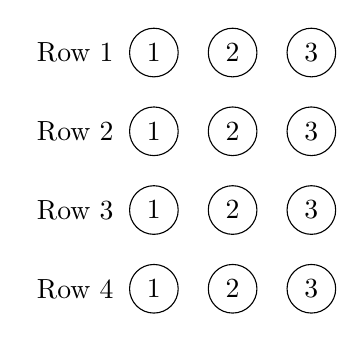
\begin{tikzpicture}
        % Draw the circles and number them
        \foreach \y in {0,1,2,3} {
            \foreach \x in {0,1,2} {
                \node[draw, circle, minimum size=0.5cm] at (\x, -\y) {\pgfmathparse{int(\x+1)}\pgfmathresult};
            }
            % Add row numbers
            \node at (-1, -\y) {Row \pgfmathparse{int(\y+1)}\pgfmathresult};
        }
    \end{tikzpicture}
\end{center}

In this grid, we have 4 rows of 3 circles each, which represents 4 × 3 = 12.
\begin{itemize}
    \item If you have 4 rows of 3 circles, you can count all the objects (3 + 3 + 3 + 3) or multiply (4 × 3 = 12).
\end{itemize}

Let’s try another example:

\textbf{Example:}
\begin{itemize}
    \item How many total buttons do you have if you arrange them in 5 rows with 6 buttons in each row?
    \item Instead of adding 6 five times, multiply: 5 × 6 = 30 buttons.
\end{itemize}

\section{What Is Division?}
Division is the reverse of multiplication. It’s used to split a total into equal parts or to see how many times one number can fit into another. For example:
\begin{itemize}
    \item You have 12 candies and want to share them equally among 4 friends. How many candies does each friend get?
\end{itemize}

This is a division problem:
\begin{itemize}
    \item 12 ÷ 4 = 3 (Each friend gets 3 candies.)
\end{itemize}

Here’s how it works:
\begin{itemize}
    \item 12 ÷ 4 means "How many groups of 4 can I make from 12?"
\end{itemize}

\subsection{Visualizing Division}
We can also use arrays and grouping to understand division. Imagine you have 12 candies, and you want to put them into groups of 4. You would end up with 3 groups of 4, which tells you that 12 ÷ 4 = 3.
\begin{center}
    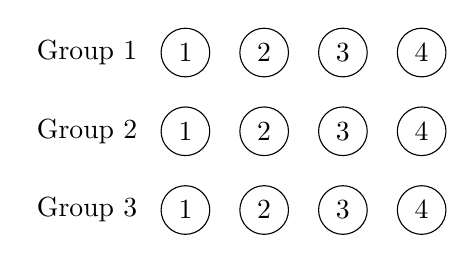
\begin{tikzpicture}
        % Draw the circles and number them
        \foreach \y in {0,1,2} {
            \foreach \x in {0,1,2,3} {
                \node[draw, circle, minimum size=0.5cm] at (\x, -\y) {\pgfmathparse{int(\x+1)}\pgfmathresult};
            }
            % Add row numbers
            \node at (-1.25, -\y) {Group \pgfmathparse{int(\y+1)}  \pgfmathresult};
        }
    \end{tikzpicture}
\end{center}

In this grid, we have 3 groups of 4 candies each, which represents 12 ÷ 4 = 3.
Another example:

\textbf{Example:}
\begin{itemize}
    \item You have 20 pieces of pizza, and you want to split them between 5 people. How many slices does each person get?
    \item Divide: 20 ÷ 5 = 4 slices per person.
\end{itemize}

\section{The Relationship Between Multiplication and Division}
Multiplication and division are opposite operations, and they are closely related. This means if you know how to multiply, you can use that knowledge to help you divide.

For example, if you know that 4 × 3 = 12, you also know:
\begin{itemize}
    \item 12 ÷ 4 = 3
    \item 12 ÷ 3 = 4
\end{itemize}

This is called the inverse relationship between multiplication and division. When you multiply two numbers to get a product, division allows you to work backwards from that product to find one of the original numbers.

\textbf{Example:}
\begin{itemize}
    \item If 7 × 8 = 56, then:
    \begin{itemize}
        \item 56 ÷ 7 = 8
        \item 56 ÷ 8 = 7
    \end{itemize}
\end{itemize}

\section{Practice Makes Perfect: Let’s Try Some Exercises!}
\subsection{Simple Multiplication:}
\begin{enumerate}
    \item 3 × 4 = \_\_\_\_
    \item 5 × 6 = \_\_\_\_
    \item 8 × 7 = \_\_\_\_
\end{enumerate}

\subsection{Simple Division:}
\begin{enumerate}
    \item 12 ÷ 4 = \_\_\_\_
    \item 20 ÷ 5 = \_\_\_\_
    \item 36 ÷ 6 = \_\_\_\_
\end{enumerate}

Remember, multiplication is repeated addition, and division is splitting into equal parts. Practice using these operations with real objects, such as grouping items or dividing things equally among friends.

\section{Everyday Examples of Multiplication and Division}
Just like addition and subtraction, multiplication and division show up in everyday life. Let’s look at some examples:
\begin{itemize}
    \item \textbf{Cooking:} If a recipe calls for 3 eggs and you’re doubling the recipe, you’ll multiply: 3 × 2 = 6 eggs.
    \item \textbf{Shopping:} You’re buying 5 packs of juice, and each pack has 6 bottles. To find the total number of bottles, multiply: 5 × 6 = 30 bottles.
    \item \textbf{Splitting Costs:} You and 3 friends are splitting the cost of a \$40 meal equally. To find out how much each person should pay, divide: 40 ÷ 4 = 10.
\end{itemize}

\section{The Properties of Multiplication}
Just like with addition, multiplication has some useful properties:

\subsection{Commutative Property of Multiplication:}
\begin{itemize}
    \item The order in which you multiply numbers doesn’t matter.
    \item For example, 3 × 5 is the same as 5 × 3. Both equal 15.
\end{itemize}

\subsection{Associative Property of Multiplication:}
\begin{itemize}
    \item When multiplying three or more numbers, the way you group them doesn’t change the result.
    \item For example, (2 × 3) × 4 = 2 × (3 × 4). Both equal 24.
\end{itemize}

\subsection{Distributive Property:}
\begin{itemize}
    \item You can break up multiplication over addition.
    \item For example, 4 × (2 + 3) is the same as (4 × 2) + (4 × 3). Both equal 20.
\end{itemize}

\section{Breaking It Down: Solving Word Problems with Multiplication and Division}
Just like with addition and subtraction, word problems are a great way to see how multiplication and division work in real life.

\textbf{Example 1: A farmer has 6 apple trees. Each tree produces 10 apples. How many apples does the farmer have in total?}
\begin{itemize}
    \item \textbf{Step 1: Identify what you know:}
        The farmer has 6 trees, and each tree produces 10 apples.
    \item \textbf{Step 2: Write the math problem:}
        6 × 10 = 60 apples.    
\end{itemize}

\textbf{Example 2: You have 24 chocolates, and you want to divide them equally among 6 people. How many chocolates does each person get?}
\begin{itemize}
    \item \textbf{Step 1: Identify what you know:}
        You have 24 chocolates, and there are 6 people.
    \item \textbf{Step 2: Write the math problem:}
        24 ÷ 6 = 4 chocolates per person.
\end{itemize}

\section{Chapter Summary}
\begin{itemize}
    \item Multiplication is repeated addition, and division is splitting into equal parts.
    \item We can visualize multiplication and division using arrays, groups, and real-world objects.
    \item Multiplication and division are related through the inverse relationship: knowing one helps you solve the other.
    \item You can use multiplication and division in everyday life, such as doubling recipes, splitting costs, or organizing objects.
    \item We learned the commutative, associative, and distributive properties of multiplication.
\end{itemize}

\section{Challenge Question:}
\begin{enumerate}
    \item You have 18 candies, and you want to put them into bags with 3 candies in each bag. How many bags do you need?
    \begin{itemize}
        \item 18 ÷ 3 = \_\_\_\_
    \end{itemize}
    \item You have 45 apples, and you want to put them into baskets with 5 apples in each basket. How many baskets do you need?
    \begin{itemize}
        \item 45 ÷ 5 = \_\_\_\_
    \end{itemize}
    \item A classroom has 30 students, and the teacher wants to divide them into groups of 6. How many groups will there be?
    \begin{itemize}
        \item 30 ÷ 6 = \_\_\_\_
    \end{itemize}
    \item You have 72 marbles and want to divide them equally among 8 friends. How many marbles does each friend get?
    \begin{itemize}
        \item 72 ÷ 8 = \_\_\_\_
    \end{itemize}
    \item A baker has 120 cookies and wants to pack them into boxes with 10 cookies each. How many boxes are needed?
    \begin{itemize}
        \item 120 ÷ 10 = \_\_\_\_
    \end{itemize}
    \item You have 56 pencils and want to distribute them equally into 7 pencil cases. How many pencils will each pencil case contain?
    \begin{itemize}
        \item 56 ÷ 7 = \_\_\_\_
    \end{itemize}
    \item A gardener has 81 flowers and wants to plant them in rows with 9 flowers each. How many rows will there be?
    \begin{itemize}
        \item 81 ÷ 9 = \_\_\_\_
    \end{itemize}
    \item You have 64 books and want to arrange them on 8 shelves equally. How many books will each shelf have?
    \begin{itemize}
        \item 64 ÷ 8 = \_\_\_\_
    \end{itemize}
    \item A factory produces 90 toys and packs them into boxes with 15 toys each. How many boxes are needed?
    \begin{itemize}
        \item 90 ÷ 15 = \_\_\_\_
    \end{itemize}
    \item You have 99 candies and want to divide them equally among 11 children. How many candies will each child get?
    \begin{itemize}
        \item 99 ÷ 11 = \_\_\_\_
    \end{itemize}
    \item A farmer has 144 eggs and wants to pack them into cartons with 12 eggs each. How many cartons are needed?
    \begin{itemize}
        \item 144 ÷ 12 = \_\_\_\_
    \end{itemize}
\end{enumerate}
